% !TeX encoding = UTF-8
% !TeX root = ../main.tex

\section{完整编译链及其实现}

\begin{frame}
    \frametitle{基于SSA的函数式编译器}
    \begin{figure}
        \centering
        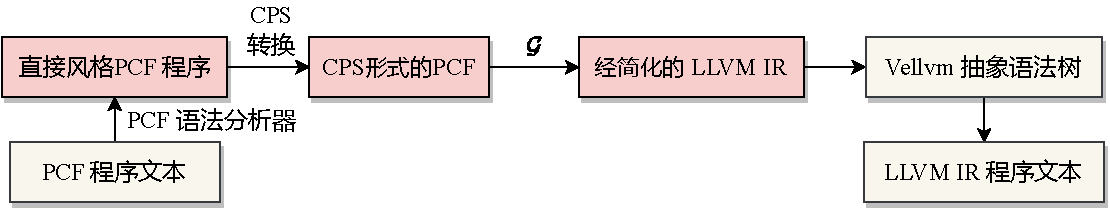
\includegraphics[width=0.9\linewidth]{figures/summary.drawio.pdf}
    \end{figure}
    \begin{itemize}
        \item 构建了一个\textcolor{Maroon}{从PCF函数式程序到LLVM IR的编译器},并对其\textcolor{Maroon}{核心编译步骤进行形式化验证}。
        \item PCF语法分析器(Parser)将PCF程序文本提取为抽象语法树。
        \item 对直接风格PCF程序进行CPS转换和CPS到SSA的转换,并进行验证。
        \item 将SSA连接到Vellvm抽象语法树,得到LLVM IR。
    \end{itemize}
\end{frame}

\begin{frame}
    \frametitle{编译器实现及代码统计}
    \begin{itemize}
        \item 主要使用交互式定理证明器\textcolor{Maroon}{Coq}实现,代码行数统计见下表(不包括所使用的CompCert中的定义和定理)。
        \item PCF语法分析器(Parser)在\textcolor{Maroon}{OCaml}中实现。
        \item 与LLVM IR的连接使用了Coq中的\textcolor{Maroon}{Vellvm}抽象语法树及其相关工具。
    \end{itemize}
    \vspace{1ex}
    
    \begin{table}
        \linespread{1.25}
        \scriptsize
        \centering
        % \vspace{-20pt}
        \begin{center}
        \begin{tabular}{|l|l|l|l|}
        \hline
        类别 & 内容 & LOC & 占比(\%) \\
        \hline
        语言定义 & PCF, CPS, SSA & 702 & 23.9 \\
        \hline
        转换算法 & \makecell[l]{PCF$\rightarrow$CPS, CPS$\rightarrow$SSA,\\SSA$\rightarrow$Vellvm LLVM IR}  & 717 & 24.5 \\
        \hline
        定理证明 & \makecell[l]{PCF$\rightarrow$CPS及CPS$\rightarrow$SSA前向模拟,\\ 前向模拟的合并及后向模拟} & 1513 & 51.6 \\
        \hline
        \end{tabular}
        \end{center}
\end{table}
\end{frame}